\begin{comment}
    \begin{itemize}
        \item Unified discussion of results
        \item How they reinforce or contrast eachother
    \end{itemize}
\end{comment}

\subsection{Simulation Study}
To validate the variational model, we conduct a simulation study.
    As the problem of multivariate extremes is the estimation of the dependence
    structure of the extremes, we focus the simulation study on on estimation of
    the angular distribution.  The simulated data is generated from a finite
    mixture of projected gammas, at varying levels of dimensionality and number
    of mixture components.  For each simulation, for a \emph{training} dataset,
    \num{1000} replicates are sampled.  For each simulation, for a 
    \emph{testing} dataset, another \num{1000} replicates are sampled using
    the same distributional parameters.

To evaluate the fidelity of the variational implementation as compared to MCMC, 
    we use a the \emph{energy score} criterion \citep{gneiting2007}, which is a
    generalization of the \emph{continuous ranked probability score} to a
    multivariate setting.  This energy score criterion takes the form
    
    In Figure~\ref{fig:energyscore} we compare rise in energy score of the fitted
    model over a \emph{baseline} energy score.  This baseline energy score is so
    named because it is the energy score between a target dataset and another
    dataset from the same generating distribution.  A value of 0 is optimal.
    \makenote{add additional model for comparison}  Note displayed scores are 
    averaged over 10 iterations \makenote{rewrite}.
    
    We see some minor loss in fidelity for the variational model as compared to 
    the MCMC model as is expected from the variational approximation.  With that
    said, the variational approximation is still quite good.

\subsection{SLOSH}

\begin{figure}[ht]
    \caption{Locations of identified sites that experienced inundation in more than 
        $5$ percent of storms.  Specifically identified are two locations of 
        interest. \makenote{Change Label to PIA} \label{map:delawarebay}}
    \centering
    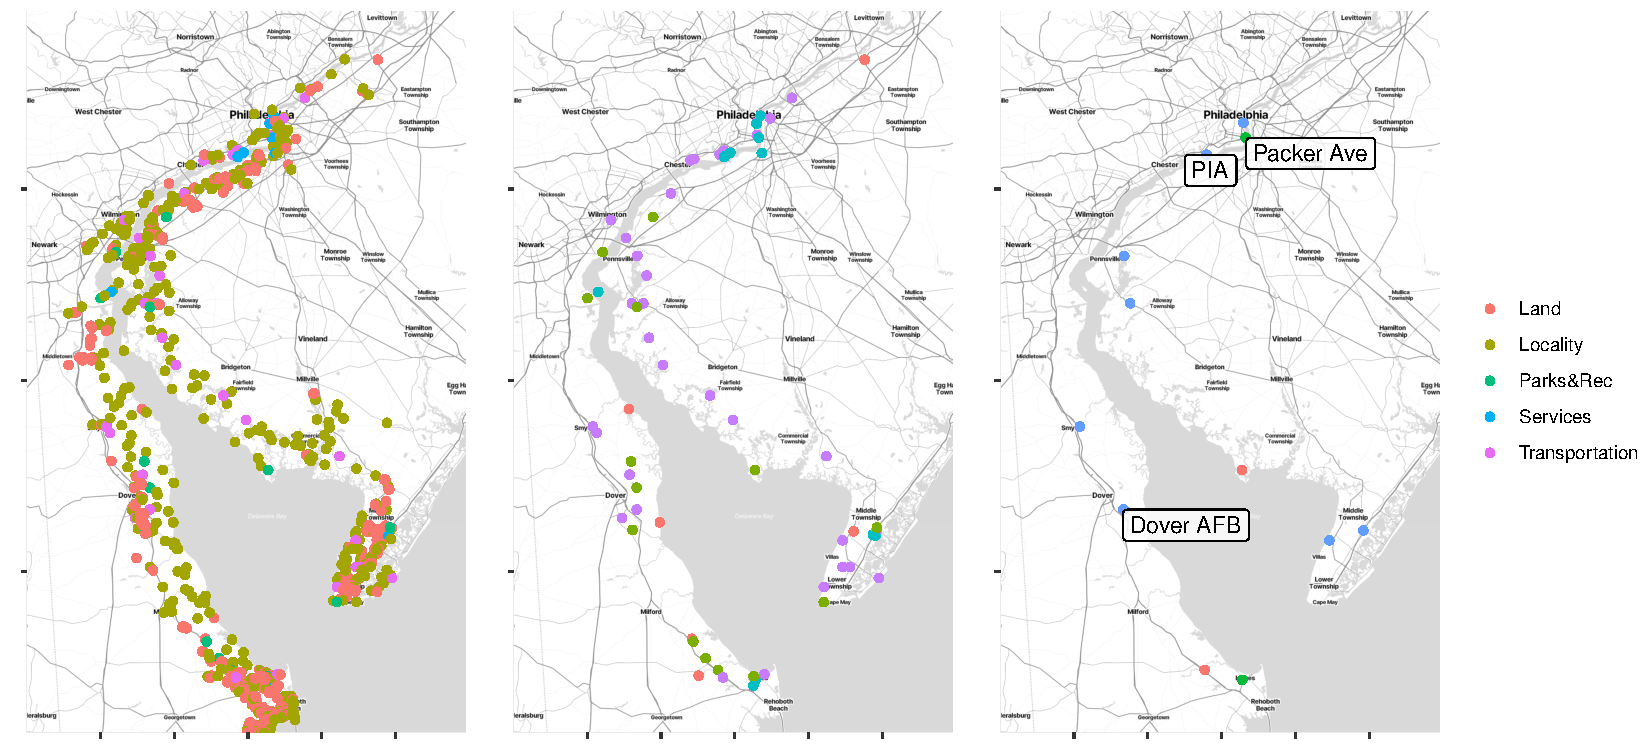
\includegraphics[height=4in]{./plots/delaware}
\end{figure}

The range of latitudes at which storms make landfall in the simulation cover a region of
    coastline surrounding the entrance of Delaware Bay \makenote{rephrase more accurate given
    data}.  Given that focus inherent in the original data, we focus our primary analysis there.
    Intersecting the original \emph{SLOSH} grid for the Delaware bay and surrounding watershed, 
    for grid cells that experienced inundation in more than 5 percent of simulations, 
    with specified locations, we identify 65 locations of interest, at which we will conduct 
    our analysis.  Figure~\ref{map:delawarebay} gives the locations of sites we identified, along
    with a classification of those sites.  Services includes emergency services, police, fire,
    and medical services.  Land includes village centers, major intersections, and named
    land features.  Transportation includes ferry landings, airports, heliports, and similar.
    Within that set, we further identify two locations of particular interest, 
    for which significant inundation can lead to catastrophic consequences:  
    Dover Air Force Base (Dover AFB), and the Philadelphia International 
    Airport (PIA). Dover AFB is situated next to Delaware Bay, with a direct approach from the
    open ocean.  PIA, on the other hand, is further upstream, adjacent to the Delaware River, 
    in the city of Philadelphia.  To reach this location, storm surge would need to backflow 
    the Delaware River a significant distance.

One difficulty with a high-dimensional model is evaluating its fidelity.  As we saw in the simulation
    study, the relative rise in energy score between a bad model and a good model shrinks as
    dimensionality increases.  This is related to the curse of dimensionality in applications like
    $k$-nearest neighbor algorithms: as the number of dimensions increases, the ratio in average
    distance between the nearest replicate, and farthest replicate in a sample will tend to approach 1.
    So distance as a measure is fundamentally flawed in a high-dimensional setting.

One thing we can do is evaluate recovery of marginal empirical CDF, using marginal
    posterior predictive CDF's under various modelling approaches.
    Having sampled $\bm{V}^{*}$ from its posterior predictive density, we can get a sample of $W_s^*$
    by inverting Equation~\eqref{eqn:standardization}.  Thus, for for $R^*\sim\text{Pareto}(1)$, 
    $Z^* = R^*\bm{V}^*$,
    \begin{equation*}
        W_s^* = a_s\left(\frac{(Z_s^*)^{\xi_s} - 1}{\xi_s}\right) + b_s
    \end{equation*}
    where $\bm{\xi}$, $\bm{a}$, and $\bm{b}$ were previously calculated.  
    For consistency with regard to the originating data, we truncate replicates 
    from the posterior predictive distribution $W_{s}^* \geq 0$.  
    \makenote{rest of paragraph potentially unnecessary}
    It can occur that the chosen marginal GP parameters are sub-optimal, as the threshold
    $b_{ts}$ may be ill-chosen.  This is an inherent weakness of choosing
    the threshold via the empirical quantile function, which creates a 
    tradeoff---to use some other method than the empirical quantile function would necessarily imply 
    non-uniform marginal probabilities of threshold exceedence, upon the assumption of which some other 
    aspects of our analysis are based. \makenote{[are they?]}

\begin{figure}[ht]
    \caption{Empirical, and posterior predictive cumulative distribution functions for marginal 
    $v$, $V^*$ (Left) and $w$, $W^*$ (Right), at Dover Air Force Base, under various modelling
    considerations.\label{plot:marginal_doverafb}\makenote{remove legend name}}
    \centering
    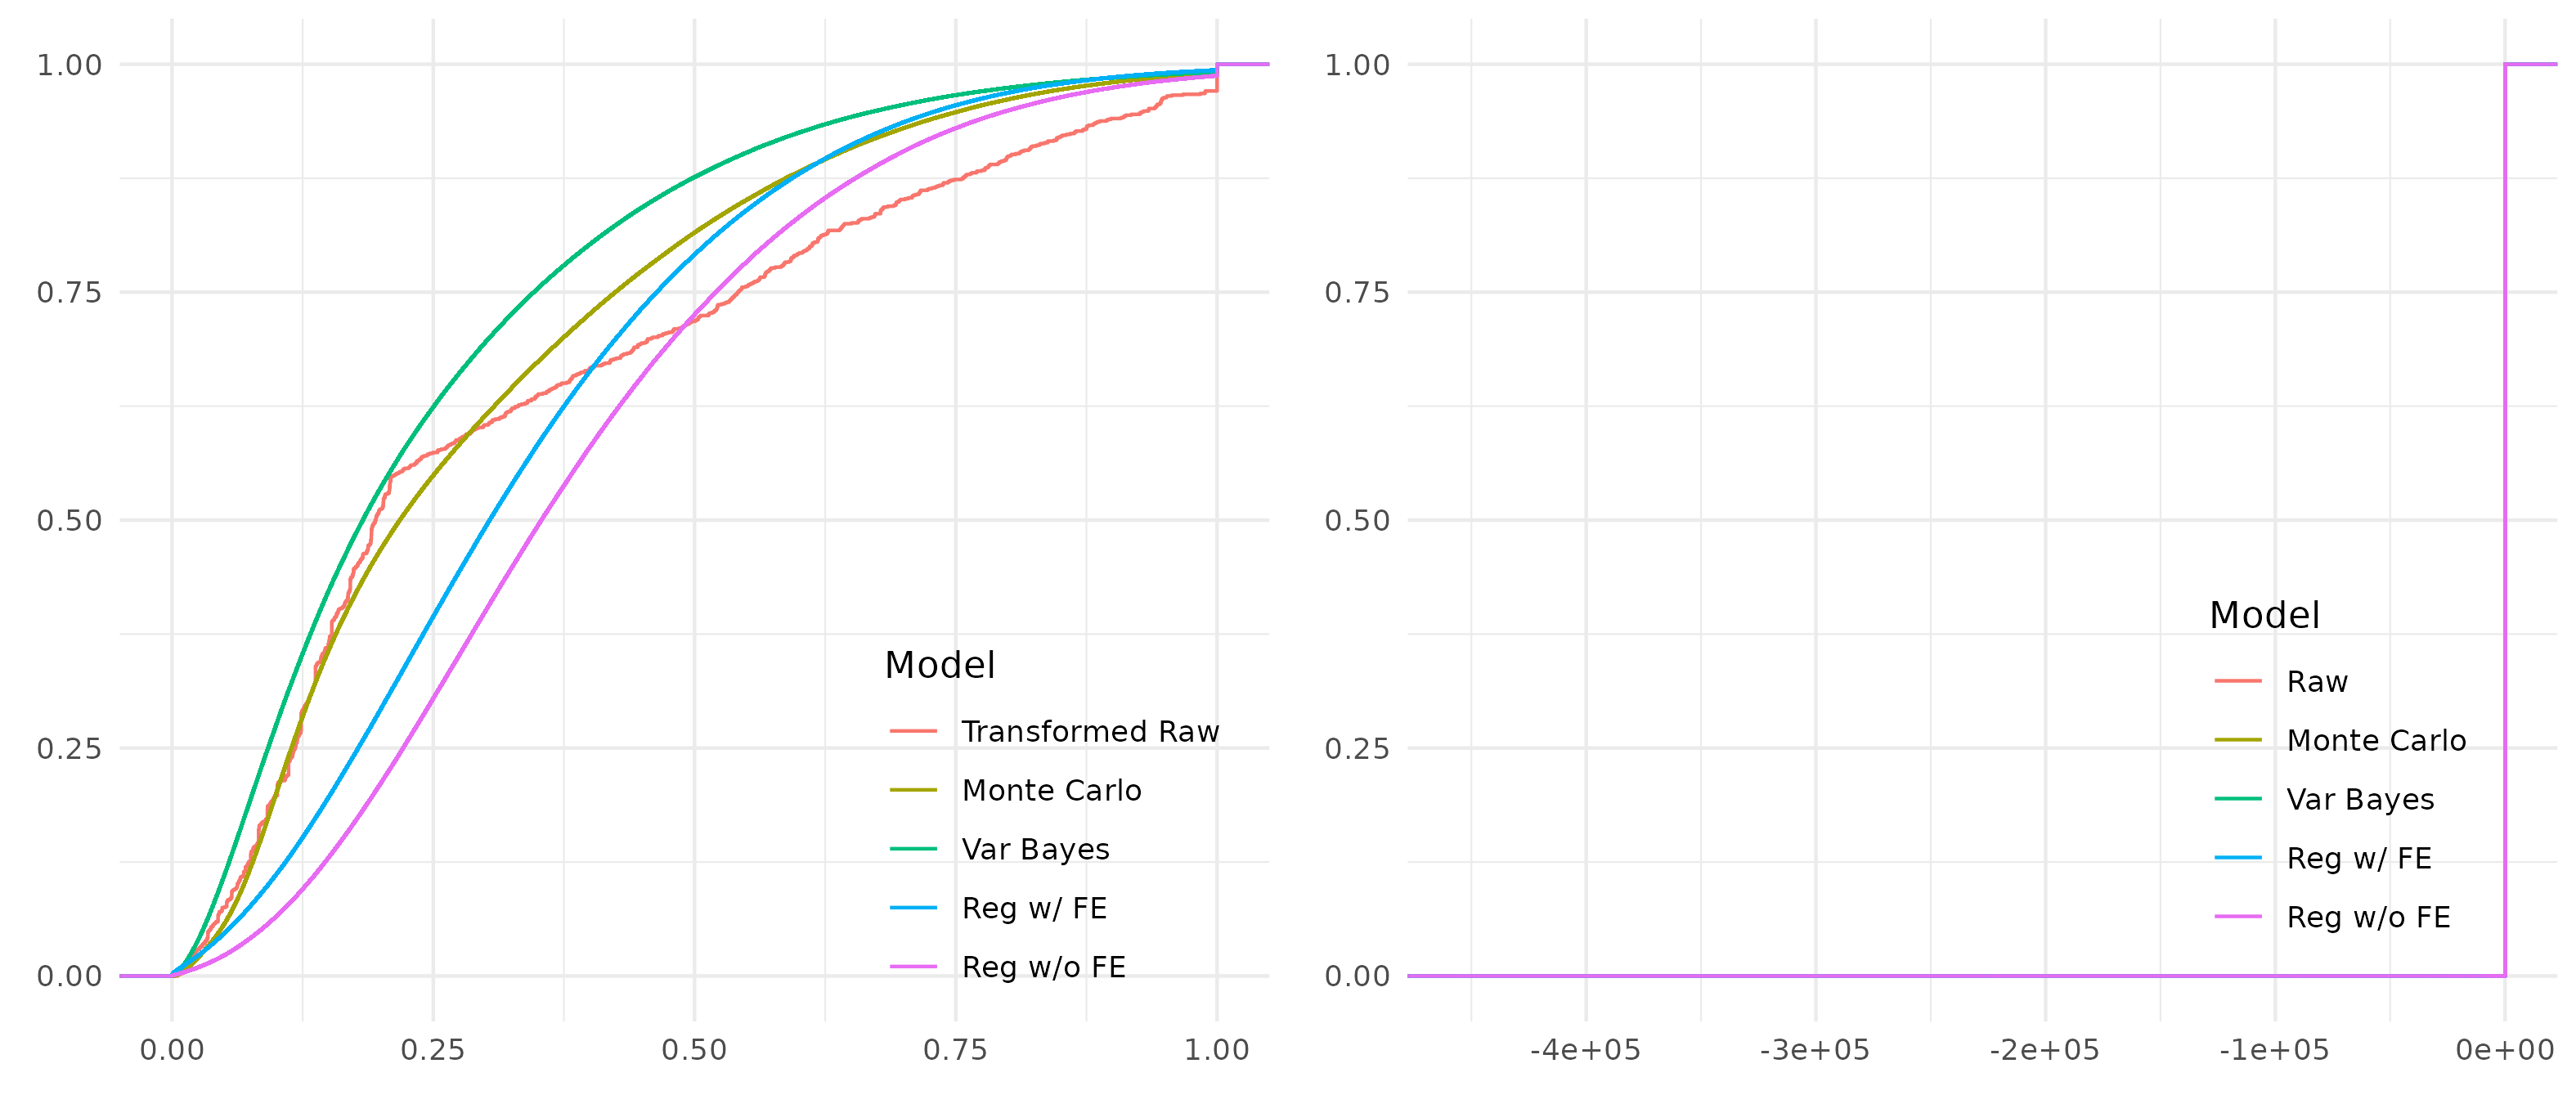
\includegraphics[width=\textwidth]{./plots/delaware_marginal_dover_afb.png}
\end{figure}

In Figure~\ref{plot:marginal_doverafb}, we observe said marginal empirical and posterior-predictive
    CDF's for storm surge at Dover Air Force Base.  As previously mentioned, this location is adjacent
    to Delaware Bay, approximately 2 miles inland, with a direct line of sight out the mouth of the
    bay towards the open ocean.  Take note in particular, that the empirical CDF of $\bm{w}_s$ shows
    that storm surge does not reach Dover AFB in approximately \num{44} percent of storms, 
    post-thresholding.

\begin{figure}[ht]
    \caption{Empirical, and posterior predictive cumulative distribution functions for marginal 
    $v$, $V^*$ (Left) and $w$, $W^*$ (Right), at Philadelphia International Airport, under 
    various modelling considerations.\label{plot:marginal_pia}\makenote{remove legend name}}
    \centering
    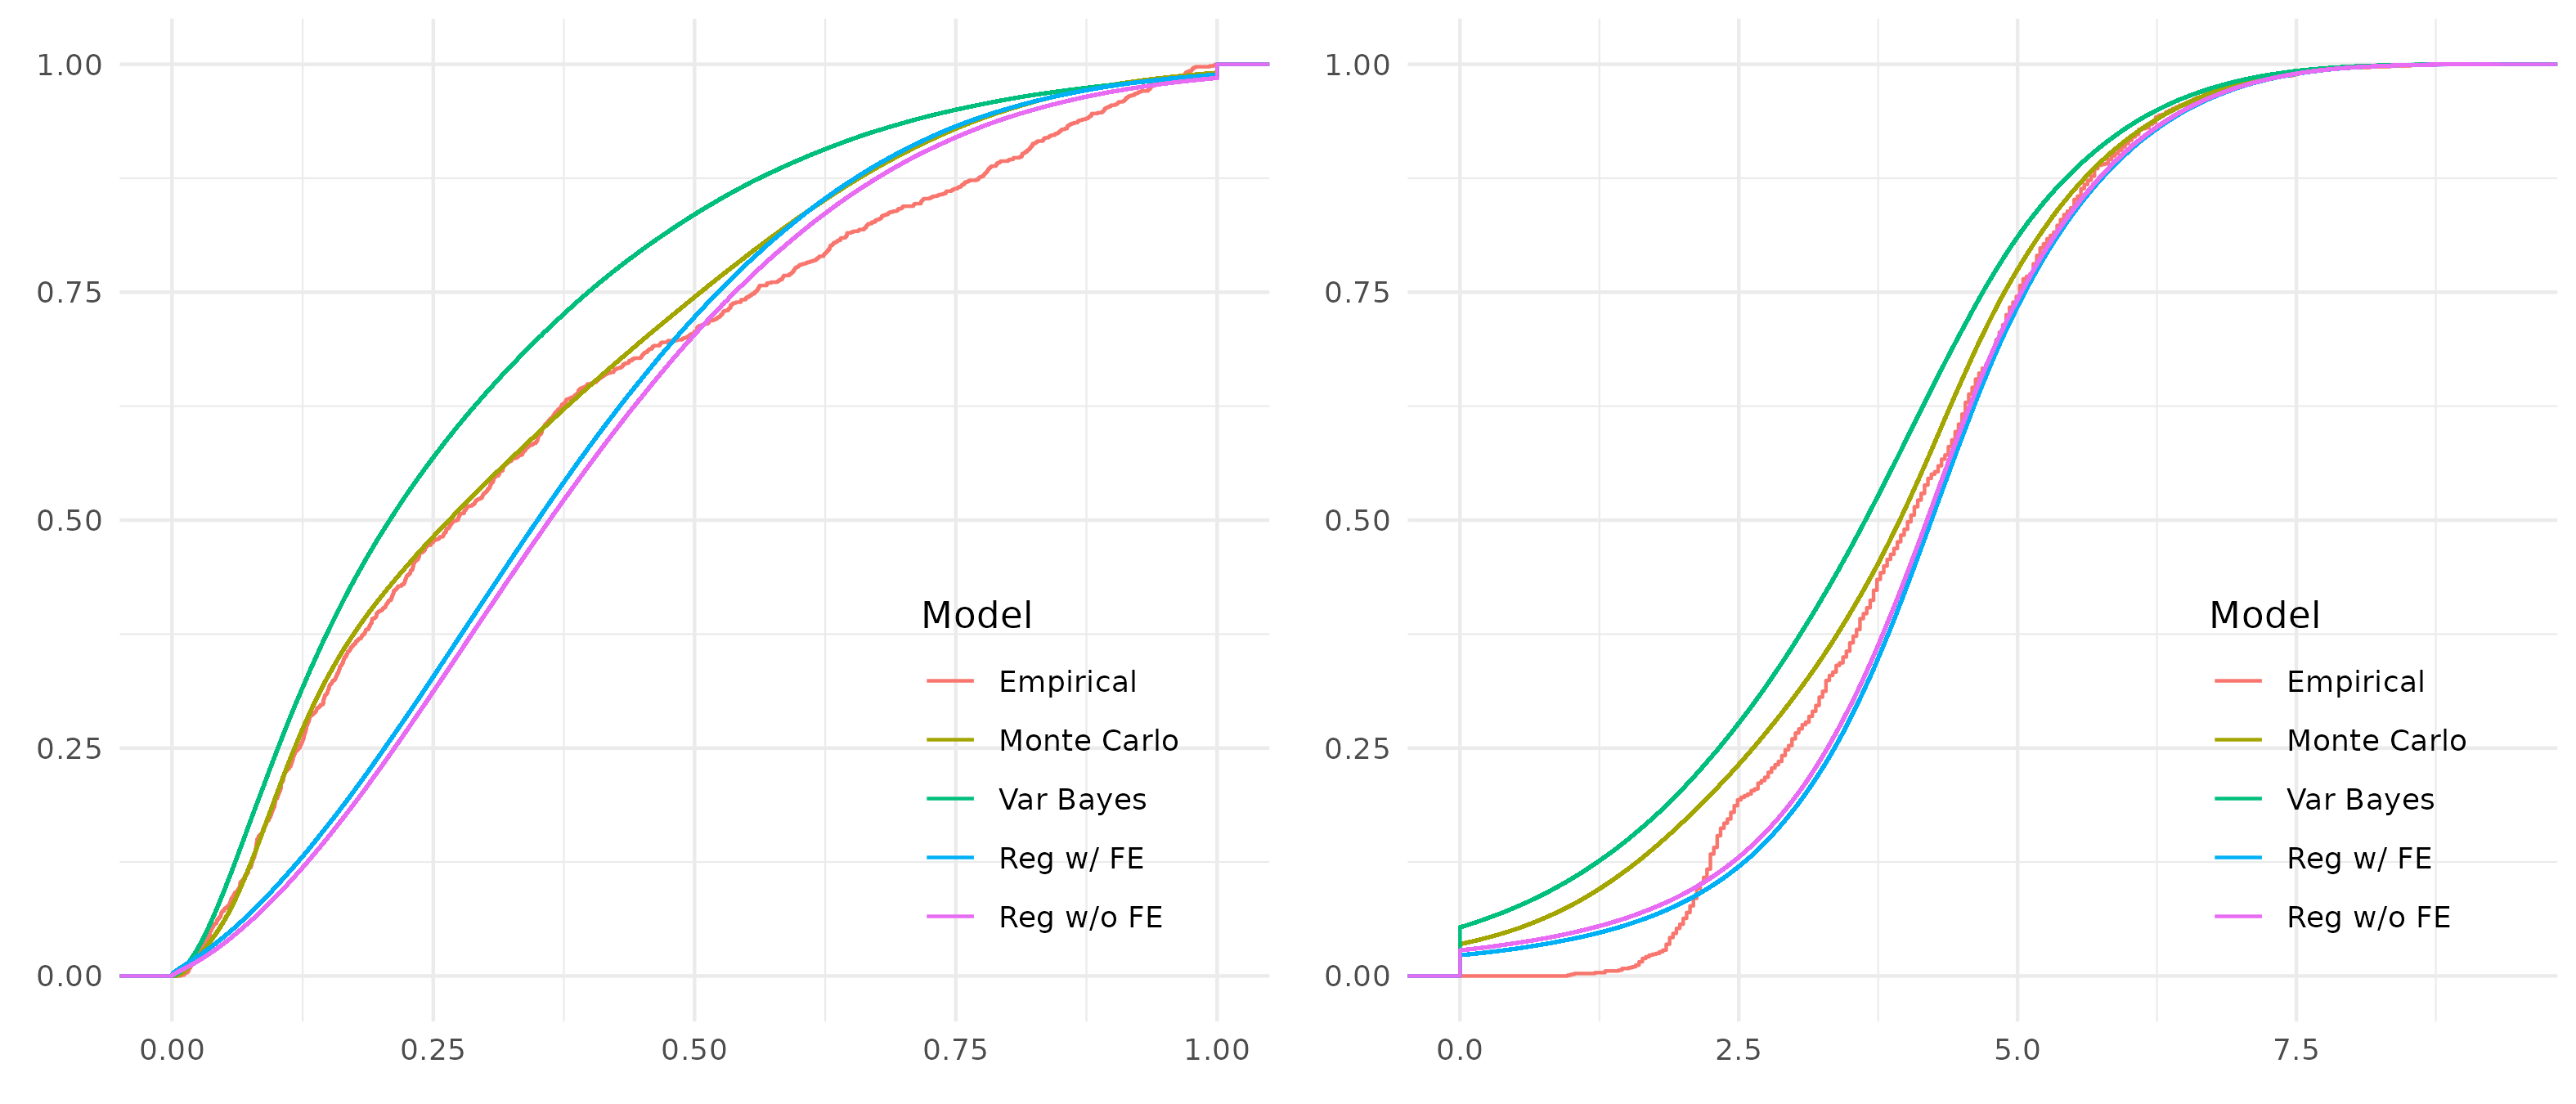
\includegraphics[width=\textwidth]{./plots/delaware_marginal_phil_ia.png}
\end{figure}

In Figure~\ref{plot:marginal_pia}, we see the same marginal CDF's, for the Philadelphia International
    Airport.  Recall, this airport is situated along the banks of the Delaware River; storm surge
    has much further to travel to reach this point, and yet it experiences inundation much more 
    frequently, owing to that its elevation is only 4 feet above sea level, rather than the 9 feet
    of Dover AFB \makenote{[confirm]}.

% latex table generated in R 4.4.1 by xtable 1.8-4 package
% Thu Oct 10 16:19:13 2024
\begin{tabular}{lrrr}
  \hline
Model & 0.9 & 0.99 & 0.999 \\ 
  \hline
Monte Carlo & 14 & 19 & 19 \\ 
  Var Bayes & 5 & 5 & 6 \\ 
  Reg w/o FE & 81 & 106 & 116 \\ 
  Reg w/ FE & 86 & 113 & 123 \\ 
   \hline
\end{tabular}


Looking at equivalent marginal plots for all locations, nearly all preserve the
    same ordering, from top-left to bottom-right: first the Variational Bayes fit of PYPG, then the 
    Monte Carlo fit of the same model, then the regression models---though the specific ordering of
    the regression models changes.  The marginal empirical CDFs tends to bounce\makenote{[rephrase]}
    between the MCMC model, and the regression models.  This means that the variational fit
    tends to consistently predict lower values than is appropriate. This permits us some insight 
    to comment what effect granularity, or the number of extant clusters, has in model fidelity.
    In Table~\ref{tab:cluster_concentration}, we see detail the number of clusters, or Pitman-Yor
    process mixture components, identified in the dataset under the specified model and fitting 
    method.  Observe the large difference between the MCMC fitting method and the VB fitting
    method. 
    \makenote{table of average $\text{E}[\alpha_s]$ under each model, as well as 
    $\text{E}\left[\frac{\alpha_s}{\lVert\bm{\alpha}\rVert_{\infty}}\right]$}

% latex table generated in R 4.4.1 by xtable 1.8-4 package
% Thu Oct 10 16:54:40 2024
\begin{tabular}{lllll}
  \hline
Slice & Var Bayes & Monte Carlo & Reg w/ FE & Reg w/o FE \\ 
  \hline
Threshold & 3 & ~ & ~ & ~ \\ 
  Delaware & 4 & 30 & ~ & ~ \\ 
  Restricted & 8 & 21 & 127 & 118 \\ 
  Critical & 11 & 51 & 30 & 22 \\ 
   \hline
\end{tabular}






    




% EOF